\chapter{Risikoanalyse und Sicherheitsmassnahmen}
\section{Schnittstellen}

\begin{table}[h!]
  \begin{tabular}{|L{0.2\textwidth}|L{0.3\textwidth}|L{0.4\textwidth}|}
      \rowcolor{puzzleblue}\color{white} Action & \color{white} Controller & \color{white} Funktion \\ [12pt]
      \hline
      index & PeopleController & Diese Schnittstelle liefert alle Personen zurück, wobei diese durch den gegebenen Filter gefiltert werden.
      Der Filter kann entweder durch die Angabe einer Filter-ID oder dem Mitgeben von Parametern im Request definiert werden.  \\
      \hline
       index & SubscriptionController & Diese Schnittstelle liefert alle Abonnemente zurück, wobei diese durch die definierten Filter
       gefiltert werden. Die Filter können über diverse Attribute bestimmt werden, im Rahmen dieser IPA sind allerdings auschliesslich die
       globalen Bedingungen zu beachten, welche auf Maillinglisten gespeichert werden, welche wiederum mehrere Abonnenmente verwalten.  \\
      \hline
    \end{tabular}
    \caption{Schnittstellen}
\end{table}

\newpage

\section{Benutzer und Datenzugriffe}
Benutzer im Hitobito besitzen immer eine Rolle. Die Rolle des Benutzers bestimmt seine Berechtigungen. Die Berechtigungen welche ein User haben kann sind:

\begin{table}[h!]
  \begin{tabular}{|L{0.3\textwidth}|L{0.8\textwidth}|}
      \rowcolor{puzzleblue}\color{white} Name & \color{white} Berechtigung \\ [12pt]
      \hline
      Group\_Full & Hat Schreib- und Leserechte auf seiner Gruppe \\
      \hline
      Group\_Read & Hat Leserechte auf seiner Gruppe  \\
      \hline
      Layer\_Full & Hat Schreib- und Leserechte auf seiner Gruppe und den Gruppen welche der Ebene dieser Gruppe unterliegen. \\
      \hline
      Layer\_Read & Hat Leserechte auf seiner Gruppe und den Gruppen welche der Ebene dieser Gruppe unterliegen. \\
      \hline
      Layer\_And\_Below\_Full & Hat Schreib- und Leserechte auf seiner Gruppe, allen Gruppen der Ebene dieser Gruppe und allen unterliegenden Ebenen. \\
      \hline
      Layer\_And\_Below\_Read & Hat Leserechte auf seiner Gruppe, allen Gruppen der Ebene dieser Gruppe und allen unterliegenden Ebenen. \\
      \hline
    \end{tabular}
    \caption{Berechtigungen}
\end{table}

\newpage

Um die Berechtigungen besser verständlich zu machen, dienen folgende Diagramme:


\subsection{Datenstruktur}
\begin{figure}[h]
  \centering
  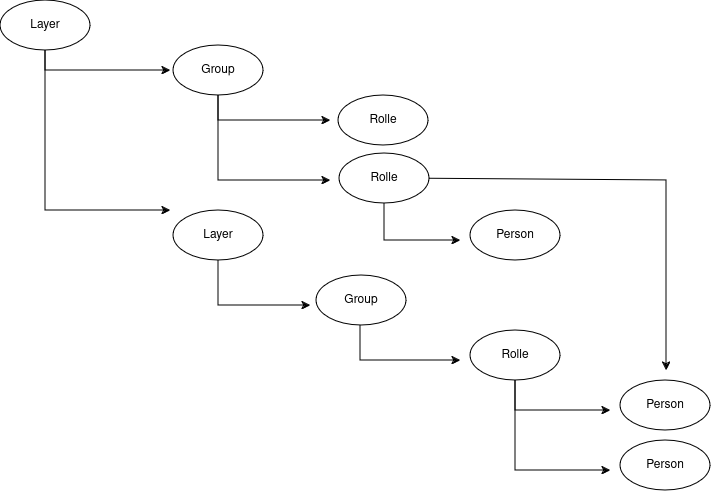
\includegraphics[width=1\textwidth,]{permissions_1.png}
  \caption{Gruppen und Ebenen, selbstgezeichnet mit Draw.io}
\end{figure}

Die Berechtigunge verwalten den Zugriff auf Layer und Gruppen. Ein Layer kann mehrere Gruppen haben,
eine Gruppe besitzt mehrere Rollen und eine Rolle kann wiederum mehrere Personen besitzen. Personen können
mehrere Rollen und somit eine Vielzahl von Berechtigungen besitzen.

\newpage

\subsection{Beispiel Zugriff Heinz}
\begin{figure}[h]
  \centering
  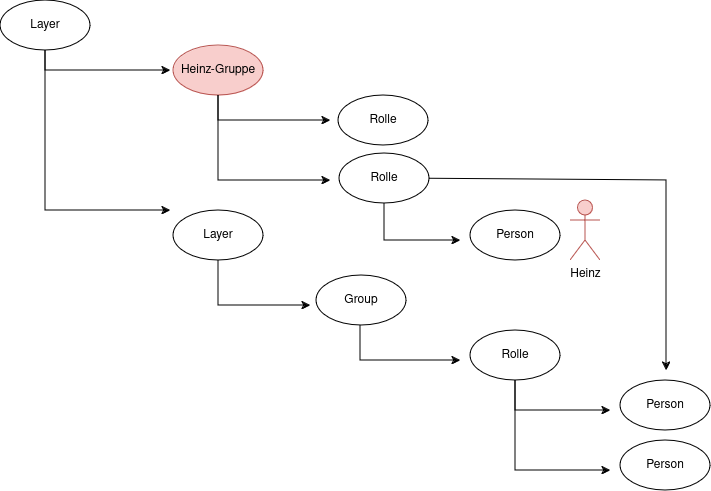
\includegraphics[width=1\textwidth,]{permissions_heinz.png}
  \caption{Beispiel Berechtigungen von Heinz, selbstgezeichnet mit Draw.io}
\end{figure}

Dieses Diagram erklärt das Beispiel der Berechtigung "Group\_Full". Wir haben einen User namens Heinz
in unserem System. Heinz besitzt eine Rolle welche mit der Heinz-Gruppe verknüpft ist. Die Rolle besitzt die Berechtigung "Group\_Full".

Dank dieser Verknüpfung besitzt Heinz Schreib- und Leserechte auf die Heinz-Gruppe.

\newpage

\subsection{Beispiel Zugriff Tim}
\begin{figure}[h]
  \centering
  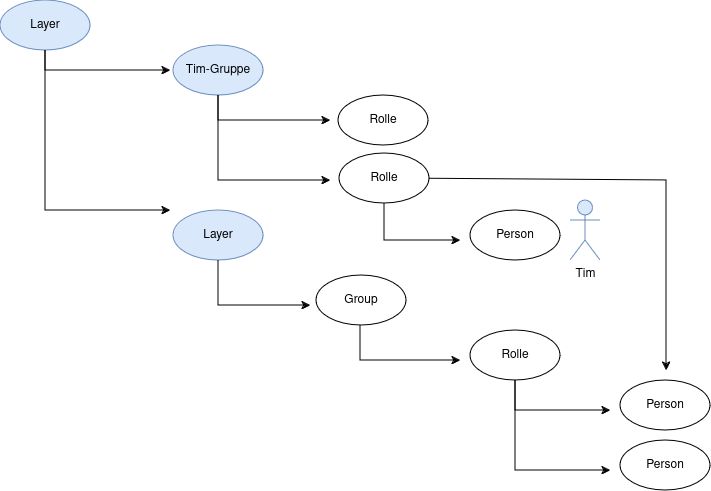
\includegraphics[width=1\textwidth,]{permissions_tim.png}
  \caption{Beispiel Berechtigungen von Tim, selbstgezeichnet mit Draw.io}
\end{figure}

Dieses Diagram erklärt das Beipsiel der Berechtigung "Layer\_Full".  Wir haben einen User names Tim in unserem System.
Tim besitzt eine Rolle welche mit der Tim-Gruppe verknüft ist. Die Rolle besitzt die Berechtigung "Layer\_Full".

Durch diese Verknüpfung hat Tim Schreib- und Leserechte auf alle Gruppen, welche dem Layer seiner Gruppe unterliegen. 

\newpage

\subsection{Beispiel Zugriff Rudolf}
\begin{figure}[h]
  \centering
  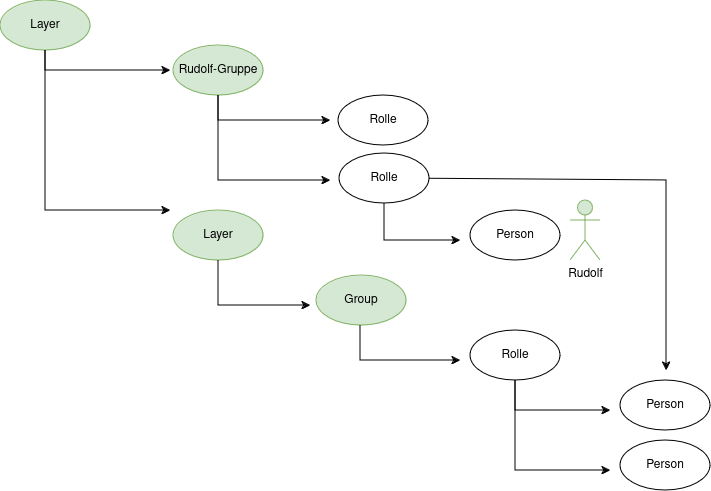
\includegraphics[width=1\textwidth,]{permissions_rudolf.png}
  \caption{Beispiel Berechtigungen von Tim, selbstgezeichnet mit Draw.io}
\end{figure}

Dieses Diagram erklärt das Beipsiel der Berechtigung "Layer\_Full\_And\_Below".  Wir haben einen User names Rudolf in unserem System.
Rudolf besitzt eine Rolle welche mit der Rudolf-Gruppe verknüft ist. Die Rolle besitzt die Berechtigung "Layer\_Full\_And\_Below".

Durch diese Verknüpfung hat Rudolf Schreib- und Leserechte auf alle Elemente, Layer und Gruppen welche dem Layer der Rudolf-Gruppe unterliegen.

\subsection{Bedeutung für die Schnittstellen}
Durch die erklärten Berechtigungen welche von den Rollen der Benutzern gegeben sind, werden die Rückgabewerte der Schnittstellen gefiltert.
Da im Rahmen dieser IPA eine Frontendanpassung gemacht wird, müssen bei der Berechtigungslogik keine Anpassungen gemacht werden. Die Berechtigungslogik wird
wie beschrieben verwendet.

\storeareas\riskvalues
\KOMAoptions{paper=a3, paper=landscape, DIV=current}
\areaset
  {\dimexpr\the\paperwidth-1cm\relax}
  {\dimexpr\the\paperheight-5.5cm\relax}
\recalctypearea

\subsection{Risikoanalyse}

\begin{table}[H]
  \begin{tabular}{ |C{0.01\textwidth}|C{0.1\textwidth}|C{0.1\textwidth}|C{0.02\textwidth}|C{0.02\textwidth}|C{0.04\textwidth}|C{0.1\textwidth}|C{0.2\textwidth}|C{0.02\textwidth}|C{0.02\textwidth}|C{0.04\textwidth}|C{0.1\textwidth}| }
      \hline
      \multirow{2}*{Nr} & \multirow{2}*{Risikobeschreibung} & \multirow{2}*{Auswirkung} & \multicolumn{4}{|l|}{Vor Massnahme}& \multirow{2}*{Massnahmen} & \multicolumn{4}{|l|}{Nach Massnahme} \\
      \cline{4-7} \cline{9-12}&&& W & S & Risiko & Handlungsweise &&  W & S & Risiko & Handlungsweise \\
      \hline 
      1 & \label{sec1} Daten ausserhalb der Berechtigung eines Benutzers werden angezeigt & Benutzer kann verbotene Informationen einsehen & W2 & S2 & \cellcolor{green}Niedrig & Risikominderung 
      & Daten werden vor dem Anzeigen im Filter anhand der Berechtigungen des Benutzers gefiltert & W1 & S1 & \cellcolor{green}Niedrig & Risikoakzeptanz \\
      \hline
      2 & \label{sec2} Benutzer kann einen Filter auf einer Ebene speichern, auf welcher er keinen Zugriff hat & Verwirrte Benutzer durch den neuen Filter & W2 & S2 & \cellcolor{green}Niedrig & Risikominderung 
      & Sicherstellen das der Benutzer nur Filter seiner Berechtigung entsprechend speichern kann. & W1 & S1 & \cellcolor{green}Niedrig & Risikoakzeptanz \\
      \hline
      3 & \label{sec3} SQL-Injection in ein Filter Eingabefeld (XSS) & Datenbank kann ausgelesen oder verändert werden & W4 & S4 & \cellcolor{red}Hoch & Risikominderung 
      & Alle Eingaben des Benutzers escapen & W2 & S1 & \cellcolor{green}Niedrig & Risikoakzeptanz \\
      \hline
      4 & \label{sec4} Bash-Injection in ein Filter Eingabefeld (XSS) & Schädliche Befehle werden serverseitig ausgeführt & W3 & S4 & \cellcolor{red}Hoch & Risikominderung 
      & Alle Eingaben des Benutzers escapen & W2 & S1 & \cellcolor{green}Niedrig & Risikoakzeptanz \\
      \hline
      5 & \label{sec5} Falsche Verwending einer Library & Schwachstelle der Library kann von Angreifern ausgenutzt werden & W2 & S3 & \cellcolor{yellow}Mttel & Risikominderung 
      & Dokumentation der Libraries gut durchgehen, diese auf Schwachstellen überprüfen
       & W2 & S2 & \cellcolor{green} Niedrig & Risikoakzeptanz \\
      \hline
  \end{tabular}
  \caption{Risikoanalyse}
\end{table}

\textbf{Schadensausmass:} \\
S1 = führt zu keinem Schaden am Projekt \\
S2 = führt zu geringem Schaden \\
S3 = hoher Schaden \\
S4 = führt zu schwerem Schaden am Projekt  \\

\textbf{Eintrittswahrscheinlichkeit:} \\
W1 = unvorstellbar \\
W2 = unwahrscheinlich \\
W3 = eher vorstellbar \\
W4 = vorstellbar \\
W5 = Eintreffen hoch \\

\restoregeometry
\riskvalues
\newpage

\section{Risikomatrix}
\begin{table}[H]
  \renewcommand{\arraystretch}{3.8}
  \begin{tabular}{*{6}{|L{0.16\textwidth}}}
      \hline
      W5 & \cellcolor{yellow}  & \cellcolor{red} &\cellcolor{red} & \cellcolor{red} \\
      \hline 
      W4 & \cellcolor{yellow} & \cellcolor{yellow} & \cellcolor{red} & \cellcolor{red} \tikz\draw[black,fill=white] circle [radius=0.2] node {3};  \\
      \hline
      W3 & \cellcolor{green} & \cellcolor{yellow} & \cellcolor{yellow} & \cellcolor{red}\tikz\draw[black,fill=white] circle [radius=0.2] node {4}; \\
      \hline 
      W2 & \cellcolor{green}\tikz\draw[black,fill=gray] circle [radius=0.2] node {3};\tikz\draw[black,fill=gray] circle [radius=0.2] node {5};\tikz\draw[black,fill=gray] circle [radius=0.2] node {4}; & \cellcolor{green} & \cellcolor{yellow}& \cellcolor{yellow}\tikz\draw[black,fill=white] circle [radius=0.2] node {5}; \cellcolor{yellow} \\
      \hline
      W1 & \cellcolor{green}\tikz\draw[black,fill=gray] circle [radius=0.2] node {1};\tikz\draw[black,fill=gray] circle [radius=0.2] node {2}; & \cellcolor{green} & \cellcolor{green} & \cellcolor{yellow} \\
      \hline
      & S1 & S2 & S3 & S4 \\
      \hline
  \end{tabular}
  \renewcommand{\arraystretch}{1}
  \caption{Risikomatrix}
\end{table}

\textbf{Legende:}\\
\tikz\draw[black,fill=white] circle [radius=0.2] node {};  Risiko ohne Massnahme \\
\tikz\draw[black,fill=gray] circle [radius=0.2] node {};  Risiko nach Massnahme \\
\tikz\draw[black,fill=green] rectangle (0.3,0.3);  Geringes Risiko \\
\tikz\draw[black,fill=yellow] rectangle (0.3,0.3);  Mittleres Risiko \\
\tikz\draw[black,fill=red] rectangle (0.3,0.3);  Hohes Risiko \\

\section{Auswertung}
Die aufgeführten Risiken sowie die entsprechenden Massnahmen wurden mit den Stakeholdern besprochen
und von ihnen abgesegnet. Durch die Bestätigung der Stakeholder, werden die Massnahmen zur Risikominderung
in der Anforderungskatalog überführt.




